% ----------------------------------------------------------------- %
%             The Speech Signal Processing Toolkit (SPTK)           %
%             developed by SPTK Working Group                       %
%             http://sp-tk.sourceforge.net/                         %
% ----------------------------------------------------------------- %
%                                                                   %
%  Copyright (c) 1984-2007  Tokyo Institute of Technology           %
%                           Interdisciplinary Graduate School of    %
%                           Science and Engineering                 %
%                                                                   %
%                1996-2015  Nagoya Institute of Technology          %
%                           Department of Computer Science          %
%                                                                   %
% All rights reserved.                                              %
%                                                                   %
% Redistribution and use in source and binary forms, with or        %
% without modification, are permitted provided that the following   %
% conditions are met:                                               %
%                                                                   %
% - Redistributions of source code must retain the above copyright  %
%   notice, this list of conditions and the following disclaimer.   %
% - Redistributions in binary form must reproduce the above         %
%   copyright notice, this list of conditions and the following     %
%   disclaimer in the documentation and/or other materials provided %
%   with the distribution.                                          %
% - Neither the name of the SPTK working group nor the names of its %
%   contributors may be used to endorse or promote products derived %
%   from this software without specific prior written permission.   %
%                                                                   %
% THIS SOFTWARE IS PROVIDED BY THE COPYRIGHT HOLDERS AND            %
% CONTRIBUTORS "AS IS" AND ANY EXPRESS OR IMPLIED WARRANTIES,       %
% INCLUDING, BUT NOT LIMITED TO, THE IMPLIED WARRANTIES OF          %
% MERCHANTABILITY AND FITNESS FOR A PARTICULAR PURPOSE ARE          %
% DISCLAIMED. IN NO EVENT SHALL THE COPYRIGHT OWNER OR CONTRIBUTORS %
% BE LIABLE FOR ANY DIRECT, INDIRECT, INCIDENTAL, SPECIAL,          %
% EXEMPLARY, OR CONSEQUENTIAL DAMAGES (INCLUDING, BUT NOT LIMITED   %
% TO, PROCUREMENT OF SUBSTITUTE GOODS OR SERVICES; LOSS OF USE,     %
% DATA, OR PROFITS; OR BUSINESS INTERRUPTION) HOWEVER CAUSED AND ON %
% ANY THEORY OF LIABILITY, WHETHER IN CONTRACT, STRICT LIABILITY,   %
% OR TORT (INCLUDING NEGLIGENCE OR OTHERWISE) ARISING IN ANY WAY    %
% OUT OF THE USE OF THIS SOFTWARE, EVEN IF ADVISED OF THE           %
% POSSIBILITY OF SUCH DAMAGE.                                       %
% ----------------------------------------------------------------- %
\hypertarget{idct}{}
\name{idct}{Inverse DCT-II}{signal processing}

\begin{synopsis}
 \item[idct] [ --l $L$ ] [ --c ] [ --d ] [ {\em infile} ]
\end{synopsis}

\begin{qsection}{DESCRIPTION}
{\em idct} calculates the Inverse Discrete Cosine Transform II (IDCT-II)
of input data in {\em infile} (or standard input),
sending the results to standard output.
The input and output data is in float format, arranged as follows.
\begin{center}
 \leavevmode
 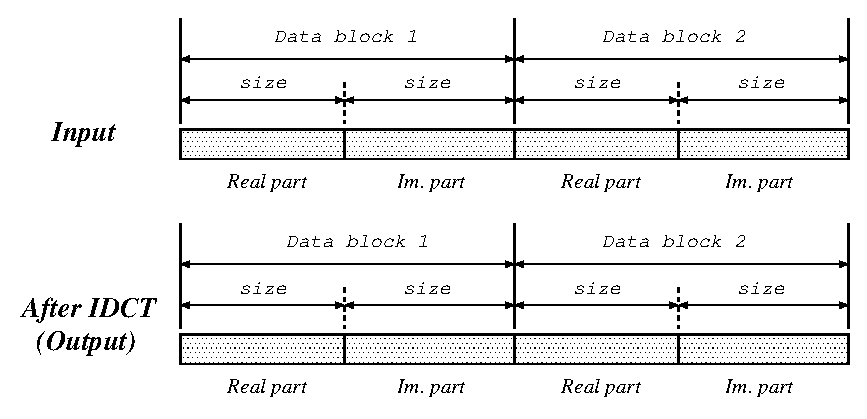
\includegraphics{fig/idct.eps}
\end{center}
The Inverse Discrete Cosine Transformation II is given by
\begin{displaymath}
 x_{l} = \sqrt{\frac{2}{L}}c_{l}\sum_{k=0}^{L-1}
 X_{k}
 \cos\left\{\frac{\pi}{L} \left( k + \frac{1}{2} \right) l\right\},
\;\;\; l = 0, 1, \cdots, L
\end{displaymath}
where
 \begin{displaymath}
c_{l}= \begin{cases}
         \;\;1 & ( 1 \le l \le L - 1 ) \\
         \;\; 1 / \sqrt{2} & (l = 0)
        \end{cases}
 \end{displaymath}
\par
\end{qsection}

\begin{options}
        \argm{l}{L}{IDCT size}{256}
        \argm{c}{}{use complex number}{FALSE}
        \argm{d}{}{don't use FFT algorithm}{FALSE}
\end{options}

\begin{qsection}{EXAMPLE}
In this example, the IDCT is evaluated from a complex-valued data file
{\em data.f} in float format
(real part: 256 points, imaginary part: 256 points),
and the output is written to {\em data.idct}:
\begin{quote}
  \verb!idct data.f -l 256 -c > data.idct!
\end{quote}
\end{qsection}

\begin{qsection}{SEE ALSO}
 \hyperlink{fft}{fft},
 \hyperlink{dct}{dct}
\end{qsection}
